\documentclass[11pt,oneside,a4paper]{article}
%define the title
\usepackage{graphicx}
\usepackage{listings}
\usepackage{setspace}
\usepackage{float}
\usepackage{titlesec}
\usepackage{amssymb}
%\usepackage{indent}
%\usepackage[labelfont=bf, textfont=normalfont, singlelinecheck=off, justification=raggedright]{caption}
% \titleformat*{\section}{\Large}
% \titleformat*{\subsection}{large}
% \titleformat*{\subsubsection}{normalsize}
\author{Group}
\title{Final_Report}
\begin{document}
\begin{titlepage}
\begin{center}
{\large \textsc{COMP2043.GRP Interim Group Report}}

\vspace{0.025\textheight} % Whitespace between the title and short horizonta
{\huge \textsc{Sequential Monte Carlo}} % Author name

\vspace{0.045\textheight}
{\huge\textsc{Team 6}}
\vspace{0.05\textheight}

{\huge\textsc{ 2017.12.7}}
\vspace{0.45\textheight}


\textbf{Supervisor:} Dr. Liang Dai
\vspace{0.045\textheight}

\textbf{Member:}
\begin{spacing}{2.0}%%�м�����Ϊdouble-space
          Hejia Qiu zy18720

          Cong Liu zy19426

          Zexi Song zy15777

          Xiang Zhang zy18743

          Kaiwen Zhang zy18672
\end{spacing}
  	\vspace{0.025\textheight}
\end{center}
\end{titlepage}
\tableofcontents
\newpage
\section{Introduction}

\subsection{Background of the Project}
Sequential Monte Carlo(SMC, also called particle filter), is a widely-used statistical sampling method, which is
used to sequentially sample from a sequence of target densities. It deals with the problem of recursively estimating
the probability density function $ p(x_t|Y_s) $.
\newline Befort the short journey of Introduction to Particle filter, a brief Background of particle filter will be explained in advanced. In our present world, the ability
of solve the problem of estimating various quantities in nonlinear dynamic systems is of paramount importance in many
practical applications. In order to understand how a system, for instance, a aircraft, a car, or a camera performs, we
need to have access to certain important quantities related with the system. However, typically we have to estimate them
based on various noisy measuremets available from the sytem due to the fact that we do not have direct access to these factors.
According to Thomas B.Schon, the state estimation problem is addressed mianly within a probabilistic framework. More specifically,
the approach is heavily affected by the Bayesian view of estimation, which implies that the complete solution to the
estimation problem is provided by the probability density function $ p(x_t|Y_s) $. This density function contains all available
information about the state variable.

\subsection{Motivation \& Wide implmentation of state estimation}
The automotive industry's focus is recently shifting from mechanics to electronics and software. This opens up factors
a great deal of interesting applications and research opportunities within the field of estimation theory.
\begin{figure}[H]
  \begin{center}
  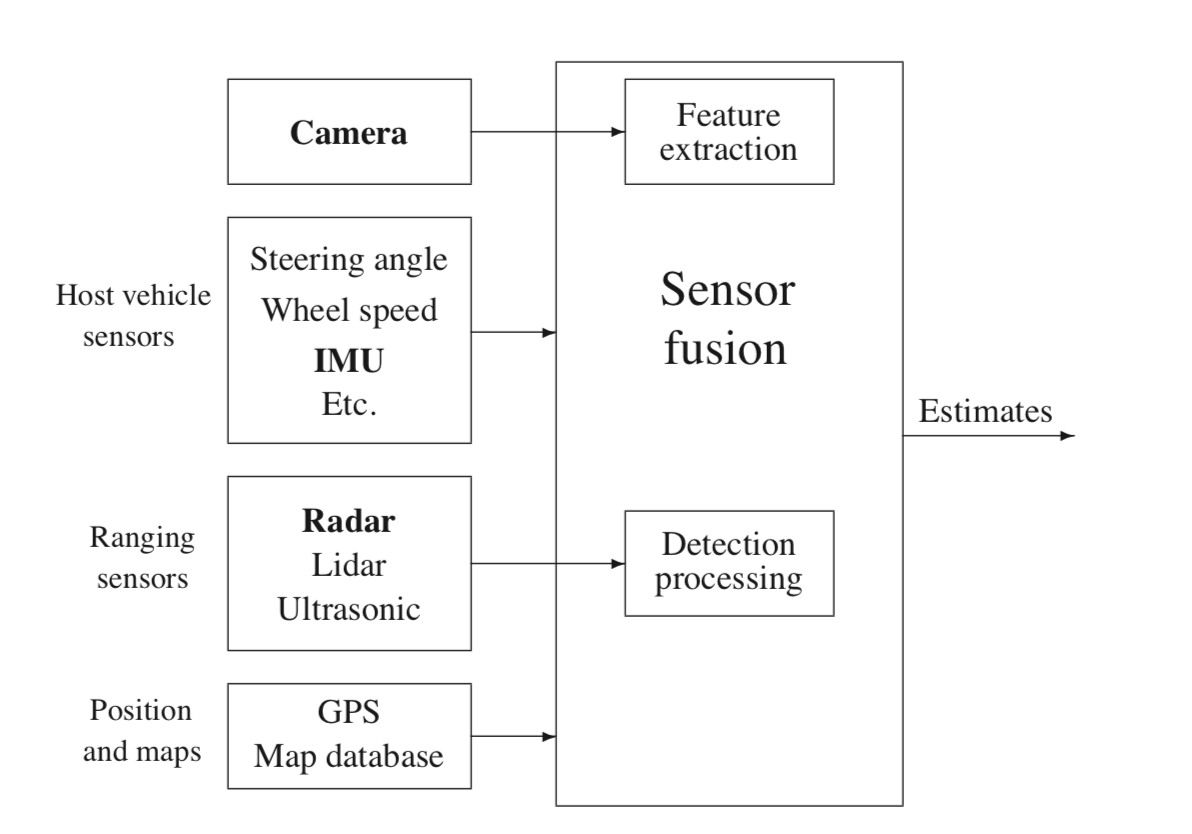
\includegraphics[height=0.3\textheight]{./source/1.png}
  \end{center}
  \caption{ The most important factors enabling future automative safety systems
  is the availablility of accurate information about the state. The process of obtaining
  this information is to a large extent dependent on a unified treament of the sensor information, as illustrated
  in this figure.}
  \label{}
\end{figure}
\subsubsection{Automotive Navigation-Example}
The objective of this study is to calculate estimates of the road geometry,
which are important in several advanced control systems such as lane guidance
and collision avoidance. The idea exemplified here follows from the general framework introduced in Figure 1.

\begin{figure}[H]
  \begin{center}
  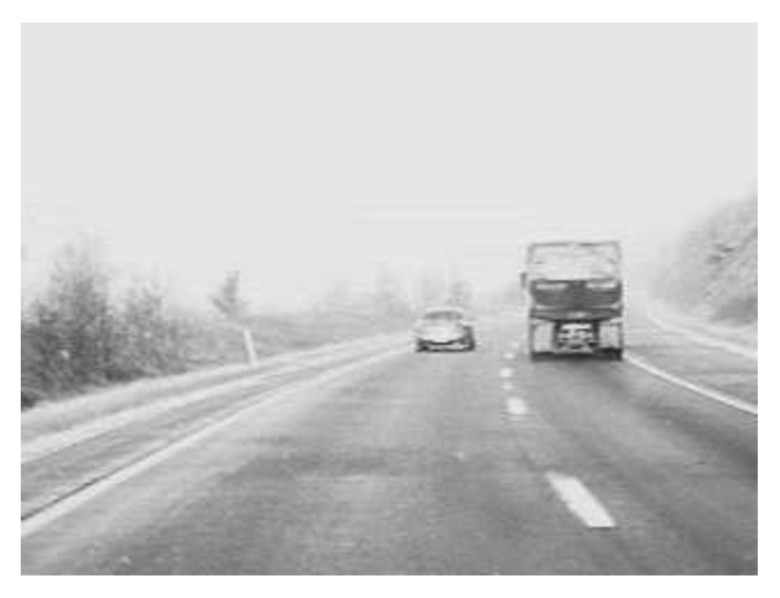
\includegraphics[height=0.3\textheight]{./source/2.png}
  \caption{when entering a curve, all vehicles start moving in the lateral direction. This information
  can be used to support the road geometry estimate.}
  \label{}
  \end{center}
\end{figure}
Here information from several sensors is used to obtain better perfomance, than separate use of the sensors would allow for.The main
assumption is that the leading vehicles will keep following their lane, and their lateral movement can thus be used to support the otherwise
difficult process of road geomtry estimation. For instance, when entering a curve as in Figure 2 the vehicles ahead will start moving to
the right and thus there is a high probability that the road is turning to the right.
Assuming that the surrounding vehicles will keep following the same lane, is in discrete-time expressed as
$y{_t+1}^i = y_{t}^i + w_t,\qquad w_t \sim \mathcal{N}(0, \mathcal{Q}_{lat}). $ Here, $y^i $ denotes the lateral
position of vehicle $i $ and $w_t $ denotes Gaussian white noise which is used to accout for model uncertainties.
The estimate of the road curvature during an exit phase of a curve is illustrated in Figure 3. The true reference
signal was generated using the method proposed by Eidehall and Gustafsson (2006).

\begin{figure}[H]
  \begin{center}
  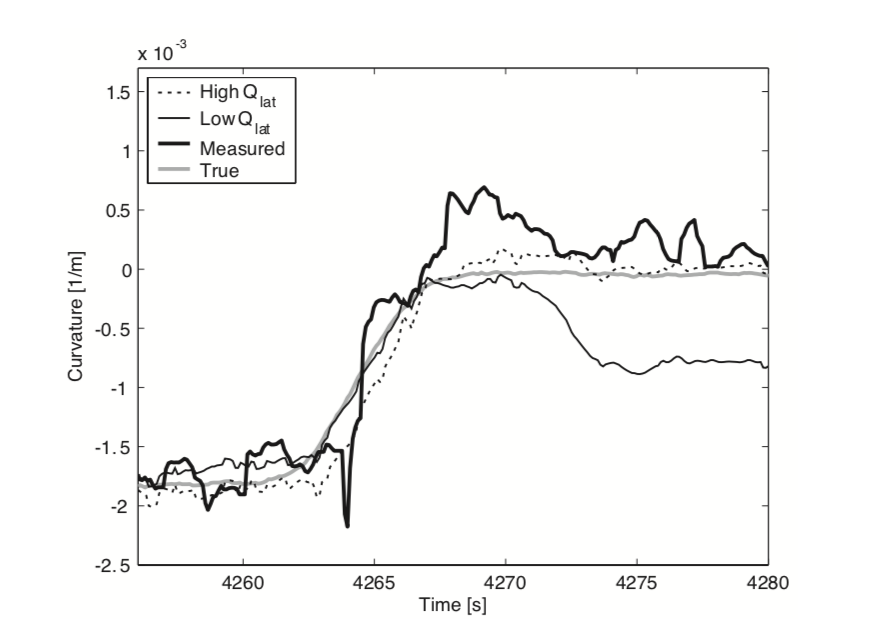
\includegraphics[height=0.3\textheight]{./source/3.png}
  \caption{Comparision of estimation performance from two filters, one with a large $\mathcal{Q}_{lat} $ and one with a small $\mathcal{Q}_{lat} $. The raw measuremet signal from the image processing
  unit is also included. Comparing this raw vision measuremet to the result from the filters clearly illustrates the power of a model based sensor fusion approach}
  \label{}
  \end{center}
\end{figure}

\subsubsection{Navigation for Augmented Reality}
\begin{figure}[H]
  \begin{center}
  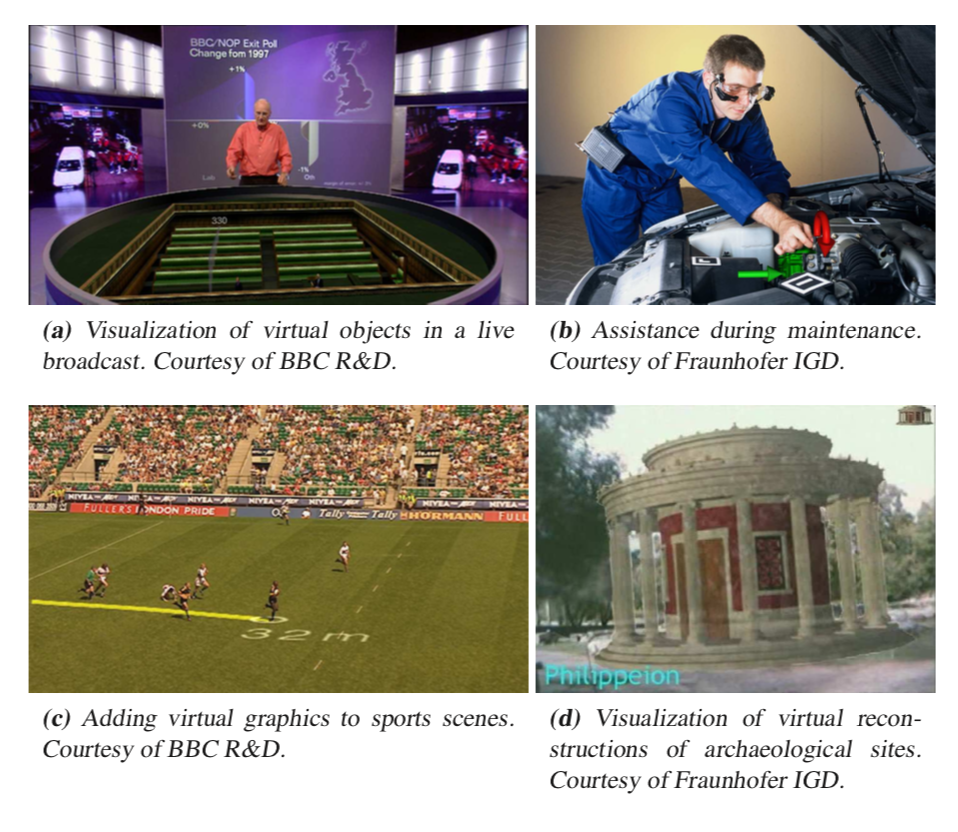
\includegraphics[height=0.35\textheight]{./source/4.png}
  \caption{Some examples illustrating the concept of augmented reality.}
  \label{}
  \end{center}
\end{figure}

\subsection{Scope of the project}
This subsection describes the scenario where the product will be used for.

\subsection{Introducing two kinds of auxiliary particle filters(APF)}
\subsubsection{Sequential Monte Carlo Methods}
As we have mentioned above that Sequential Monte Carlo methods, or particle methods, provide the solution for state estimation. Then, what does it
constitue? It is constituted by a combination of sequential importance sampling and resampling. The key idea underlying the particle methods is to represent
the probability density function by a set of samples(also referred to as particles, hence the name particle methods) and its associated weights.
The density function $p(x_{t}|Y_s) $ is approximated with an empirial density function,
\begin{equation}
p(x_{t}|Y_s) \approx \sum_{i=1}^M\tilde{q}_t^{(i)}\delta(x_t - x_{t|s}^{(i)}), \qquad \sum_{i=1}^{M}\tilde{q}_{t}^{(i)} = 1, \qquad \tilde{q}_{t}^{(i)} \geq 0, \forall{i}
\end{equation}
where $\delta(\cdot) $ represents the Dirac delta function and $\tilde{q}_{t}^{(i)} $ denotes the weight associated with particle $x_{t|s}^{(i)} $. For intuition we can think of each
particle $x_{t}^{i} $ as a possible system state and the corresponding weight $\tilde{q}_{t}^{(i)} $ contains information about how probable that particular state is.
\begin{figure}[H]
  \begin{center}
  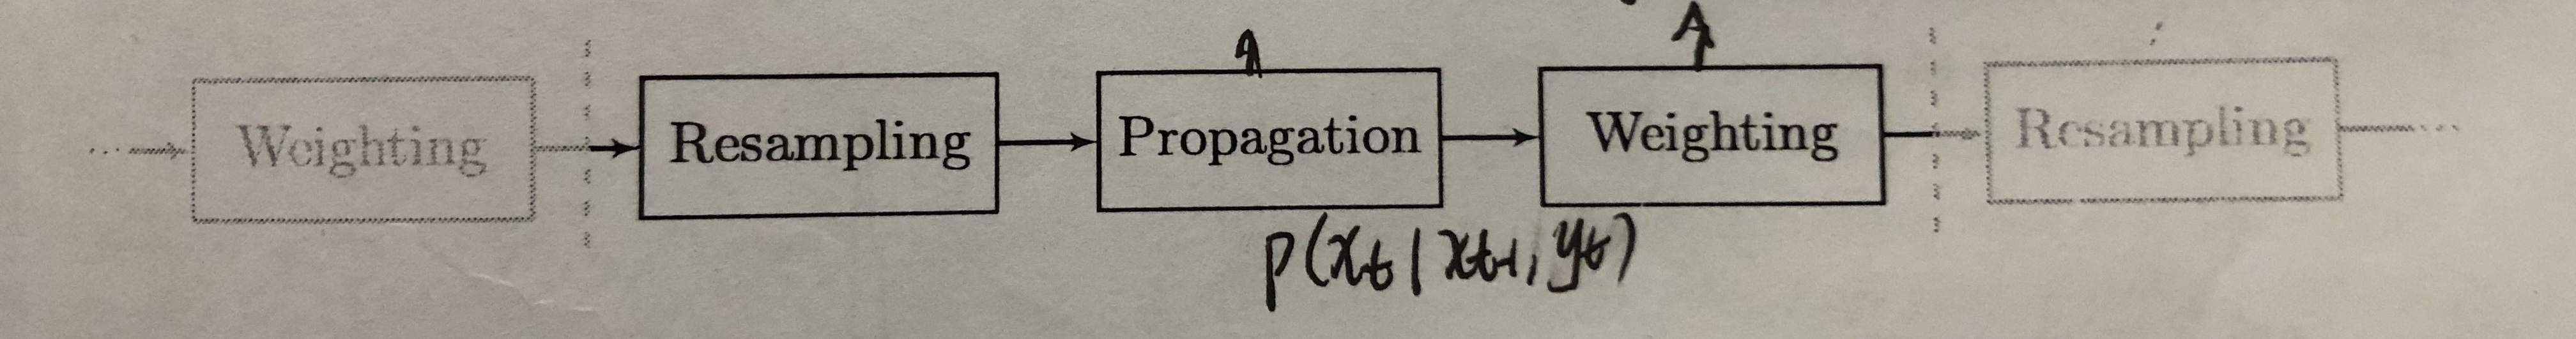
\includegraphics[width=0.9\textwidth]{./source/5.JPG}
  \caption{Illustrating the three parts making up sequential Monte Carlo}
  \label{}
  \end{center}
\end{figure}

\subsubsection{Auxiliary particle filter(APF)}
As a principled solution to compute the filtering PDFs $ \lbracep(x_t|y_{1:t})\rbrace $ sequentially in time is provided by the following
two recursively equations:\\
\begin{equation}
p(x_{t} | y_{1:t}) = p(x_t | y_t, y_{1:t-1}) = \frac{p(y_t|x_t)p(x_t|y_{1:t-1})}{p(y_t|y_{1:t-1})}
\end{equation}
\begin{equation}
p(x_{t} | y_{1:t-1}) = \int p(x_t|x_{t-1})p(x_{t-1}|y_{1:t-1}) d_{x_{t-1}}
\end{equation}
These two equations are coming from Forward filtering. The explaination will be included in the Appendixes in detail. Further, the main barrier here is the integral in equation (3), which is in general
not analytically tractable. Nevertheless, the integral can be approximated using an importance sampler targeting the filtering distribution at time $ t-1 $. This give us the impetus to proceed in an inductive
fashion. Thus,assuming we have an empirial approximation of the filtering distribution at time t-1, constituted by N weighted samples, $\{ x_{t-1}^i, w_{t-1}^i \}_{i=1}^{N} $, i.e.
\begin{equation}
\hat{p}^N(x_{t-1}|y_{1:t-1}) = \sum_{i=1}^N w_{t-1}^i\delta_{x_{t-1}^i}(x_{t-1})
\end{equation}
At time $t = 1 $, it is able to obtain a point-mass approximation according to eqution (4), by targeting $p(x_{1}|y_{1}) \propto p(y_{1}|x_{1})\mu{(x_{1})} $ with an importance sampler. Inserting the approximation
$\hat{p}^N(x_{t-1}|y_{1:t-1}) $ into equaiton(3), result in
\begin{equation}
\hat{p}^N(x_{t}|y_{1:t-1}) = \int p(x_{t}|x_{t-1}) \sum_{i=1}^{N} w_{t-1}^{i}\delta_{x_{t-1}^{i}}(x_{t-1})d_{x_{t-1}} = \sum_{i=1}^{N}w_{t-1}^{i}p(x_{t}|x_{t-1}^{i})
\end{equation}
Using equation(5) and equation(2), we can evaluate an approximation of the filtering PDF $p(x_t|y_{1:t} $ up to proportionality
\begin{equation}
p(x_{t}|y_{1:t}) \approx \frac{1}{p(y_t|y_{1:t-1})} \sum_{i=1}^N w_{t-1}^i p(y_t|x_t)p(x_t|x_{t-1}^i)
\end{equation}
As for this opens up for targeting $p(x_{t}|y_{1:t}) $ with an importance sampler. Then, choosing a similar type of mixture
as proposal density, namely
\begin{equation}
q(x_{t}|y_{1:t}) = \sum_{i=1}^N w_{t-1}^i q(x_t|x_{t-1}^i,y_t)
\end{equation}
There are many different options when it comes to choosing the component $q(x_{t}|x_{t-1}^{i}, y_{t}) $ in this mixture. Note that, in general, the proposal density at time $t $ is allowed to depend on the current
observation $y_{t} $, as indicated by the notation used in equation (7). Therefore, Using auxiliary variable in the form of a discrete random variable $a_{t} $ which takes values on the set of integers $\{ 1,...,N\} $ in the $q(x_t|y_{1:t}) $ can take $y_{t} $ into account, which make use of this information already when simulating
the particles $\{ x_{t}^{i} \}_{i=1}^{N} $, to increase the probability of producing samples in the most relevant parts of the state space. This is why we indicate a possible dependence on $y_{t} $ in the mixture components of
the proposal density in (7).The key in this development is to target the joint distribution of $(x_{t}, a_{t}) $ with an importance sampler, instead of directly targeting the marginal
distribution of $x_{t} $\\
Analogously to above, the mixture proposal (7) can be interpreted as a joint proposal distribution for the pair $(x_{t}, a_{t}) $, given by
\begin{equation}
q(x_{t}, a_{t} | y_{1:t}) = w_{t-1}^{a_t}q(x_{t}|x_{t-1}^{a_{t}}, y_{t})
\end{equation}
Here, $a_{t} $ should be thought of as an index selecting one of the componets in the sum (7).
Generating, independently, N realizations from this joint proposal distribution can be done as follows.\\
\flushleft
\begin{enumerate}
\item Sample the ancestor indices $ \{ a_{t}^{i} \}_{i=1}^{N} $ according to
\begin{equation}
\mathbb{P} (A_{t} = i \arrowvert \{ x_{t-1}^{j}, w_{t-1}^{j} \}_{j=1}^{N} ) = w_{t-1}^{i} \qquad i = 1,...,N
\end{equation}
This corresponds to the resampling step of the algorithm. The resampled particles are given as $ \bar{x}_{t-1}^{i} = x_{t-1}^{a_{t}^{i}} $ for $ i = 1,...,N $.
\item Propagate the particles to time t by simulating $x_{t}^{i} \backsim q(x_{t}| \bar{x}_{t-1}^{i}, y_{t}) $ for $i = 1,...,N $
\end{enumerate}
The advantage of explicitly introducing and implmenting auxiliary variable lies in the computation of the importance weight. From (6),
we have that the joint target distribution for $(x_{t}, a_{t}) $ is proportional to what called unnormalized joint target density:
\begin{equation}
w_{t-1}^{a_{t}}p(y_{t}|x_{t})p(x_{t}|x_{t-1}^{a_{t}})
\end{equation}
In fact, it is possible to use the information available in the current observation $y_{t} $, not only when proposing the new state $x_{t} $, but also when proposing its ancestor index $a_{t} $. The principle is that we can thereby increase the probability of resampling particles at time $t-1 $ that are in
agreement with the observation $y_{t} $. \\
It is free to use any proposal distribution that we find appropriate to obtain the pair $(x_{t}, a_{t}) $ (Thomas B. Schon, Fredrik Lindsten, 2017). For example, let $V $ be the function that will be used to adapt the proposal distribution for the ancestor indices. For each particle
, i.e. for $i = 1,...,N $, we then compute the quantities
\begin{equation}
  v_{t-1}^{i} := v(x_{t-1}^{i}, y_{t}),
\end{equation}
referred to as adjustment multipliers. The adjustment multipliers are used to construct a proposal distribution for the ancestor index variable $a_{t} $
\begin{equation}
\mathbb{P} (A_{t} = i \arrowvert \{ x_{t-1}^{j}, w_{t-1}^{j} \}_{j=1}^{N} , y_{t} ) = \frac{w_{t-1}^{i} V_{t-1}^{i}}{\sum_{t=1}^{N} w_{t-1}^{l} v_{t-1}^{l}} \qquad i = 1,...,N
\end{equation}
From the above expression, it is clear that v acts as adjusting the original weights $w $ via multiplication. The underlying ideas of implementation of adjustment multipliers is that by carefully choosing the function $v $, we can adapt the sampling of the ancestor
indices in (16) to make use of the information available in the current measuremet $y_{t} $ \\
Then, we get the following expression for the $i $ importance weight as the use of adjustment multipliers:
\begin{equation}
\bar{w}_{t}^{i} = w(x_{t-1}, x_{t}, y_{t}) = \frac{w_{t-1}^{a_{t}^{i}} p(y_{t}|x_{t}^{i}) p(x_{t}^{i}|x_{t-1}^{a_{t}^{i}})}{w_{t-1}^{a_{t}^{i}} v(\bar{x}_{t-1}, y_{t}) q(x_{t}^{i}|x_{t-1}^{a_{t}^{i}}, y_{t})}
\end{equation}
This completes the algorithm, since these weighted particles in turn can be used to approximate the filtering PDF at
time t+1, then at time t+2 and so on.


\subsubsection{Bootstrap particle filter}
After we have known the Auxiliary particle filter, a pragmatic solution for bootstrap particle filter is to choose the proposal density according to
\begin{equation}
w_{t-1}^{a_{t}^{i}} v_{t-1}^{a_{t}} = w_{t-1}^{a_{t}},
\end{equation}
\begin{equation}
q(x_{t}|x_{t-1}^{a_{t}}, y_{t}) = p(x_{t}|x_{t-1}^{j}),
\end{equation}
\begin{equation}
q(x_{t}, a_{t} | y_{1:t}) = \sum_{j=1}^{N}w_{t-1}^{j}p(x_{t}|x_{t-1}^{j})
\end{equation} \\
Therefore, From (6) and (7) it follows that the weight function is given by
\begin{equation}
\bar{w}_{t}^{i} = \frac{p(x_{t}, a_{t}|y_{1:t})}{q(x_{t}, a_{t}|y_{1:t})} = p(y_{t}|x_{t})
\end{equation}
This completes the algorithm.
\begin{figure}[H]
  \begin{center}
  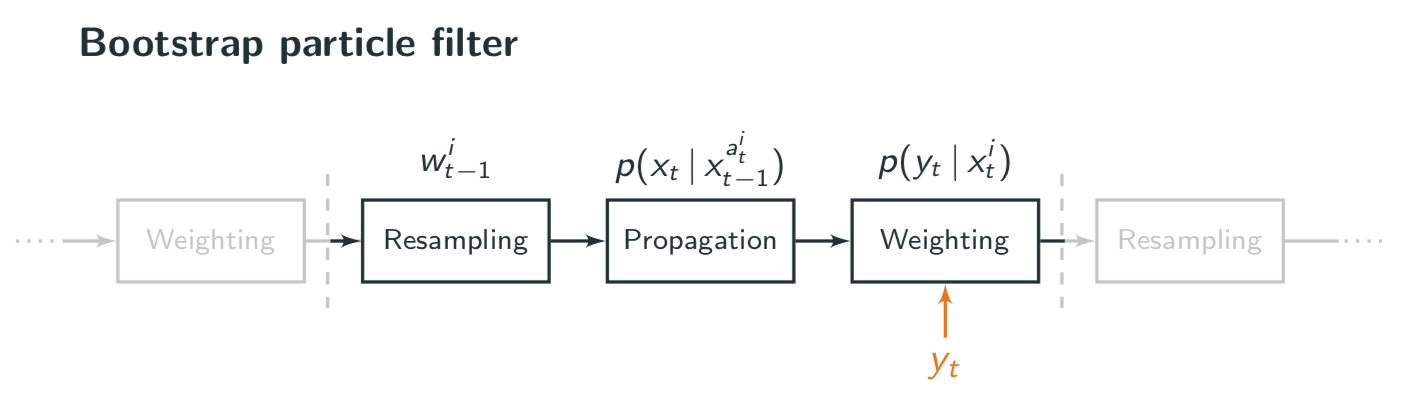
\includegraphics[width=0.9\textwidth]{./source/6.png}
  \caption{}
  \end{center}
  \label{}
\end{figure}
\subsubsection{Fully adapted particle filter}
In order to adapt the proposals to the information that is available in the current observation $y_{t} $. A nature choice as for the proposal for the state $x_{t} $ is to use
\begin{equation}
  q(x_{t}|x_{t-1}, y_{t}) = p(x_{t}|x_{t-1}, y_{t}),
\end{equation}
From Bayes'rule, we can write
\begin{equation}
  p(x_{t}|x_{t-1}, y_{t}) = \frac{p(y_{t}|x_{t}) p(x_{t}|x_{t-1})}{p(y_{t}|x_{t-1})},
\end{equation}
Plugging this expression into the denominator of equation (13) we obtain
\begin{equation}
\bar{w}_{t}^{i} = w(x_{t-1}, x_{t}, y_{t}) = \frac{p(y_{t} | x_{t-1})}{v(x_{t-1}, y_{t})},
\end{equation}
When it confront the choice to decide the adjustment multipliers. In particular, we see the choice $v(x_{t-1}, y_{t}) = p(y_{t}|x_{t-1}) $ will lead to a weight function that is identically equal to 1. In other word, we obtain particles that are generated in such a way that they are equally informative about the
target distribution.
\begin{equation}
  \bar{w}_{t}^{i} = 1.
\end{equation}
This completes the algorithm.
\begin{figure}[H]
  \begin{center}
  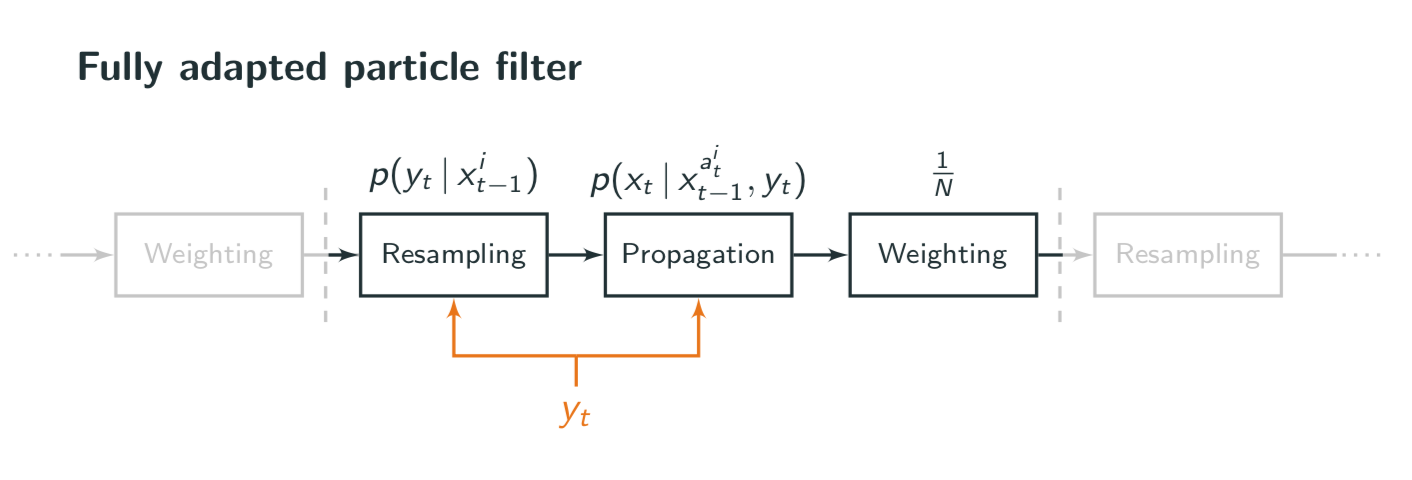
\includegraphics[width=0.9\textwidth]{./source/7.png}
  \caption{}
  \label{}
  \end{center}
\end{figure}















\end{document}
